\begin{figure}[H]
	\centering
	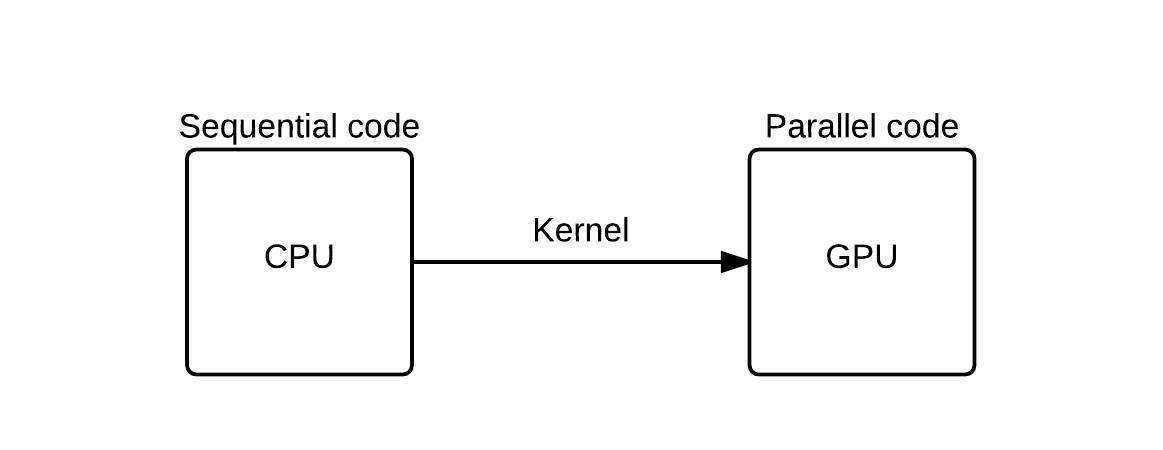
\includegraphics[width=\textwidth]{system_overview/diagrams/programming_model_cpu_gpu.png}
	\caption{Relationship between CPU and GPU code.}
	\label{fig:programming_model_cpu_gpu}
\end{figure}
Programming for Demolicious will seem familiar for readers with programming experience from technology like CUDA or OpenCL. 
Many applications can be divided into sequential and parallel parts, where each part can benefit from different execution models. \todo{Is this a word<Execution model>?}
On the Demolicious system, the sequential parts of a program will be run by the CPU, and the parallel parts can be performed by the GPU through kernels.
A kernel is a simple program meant to be executed by multiple threads.
The kernels are usually uploaded to the GPU at the start of the program, and then executed when requested by the CPU.
This architecture is well suited for highly parallel tasks such as graphics.

\subsection{Kernels}
As kernels are meant to be executed in very high volumes on the GPU, 
To vary output from different kernels, each thread is assigned a unique thread id.
These can be used for address offsets when writing to memory,
color variations, or ANYTHING u can imagen.
To keep the architecture simple, kernels support a fairly limited instruction set.
Most notably, all kernels are purely linear, meaning they cannot do any branches or jumps.
All hope is not lost, though. Mask, etc.

\subsection{Memories}

\begin{figure}[H]
	\centering
	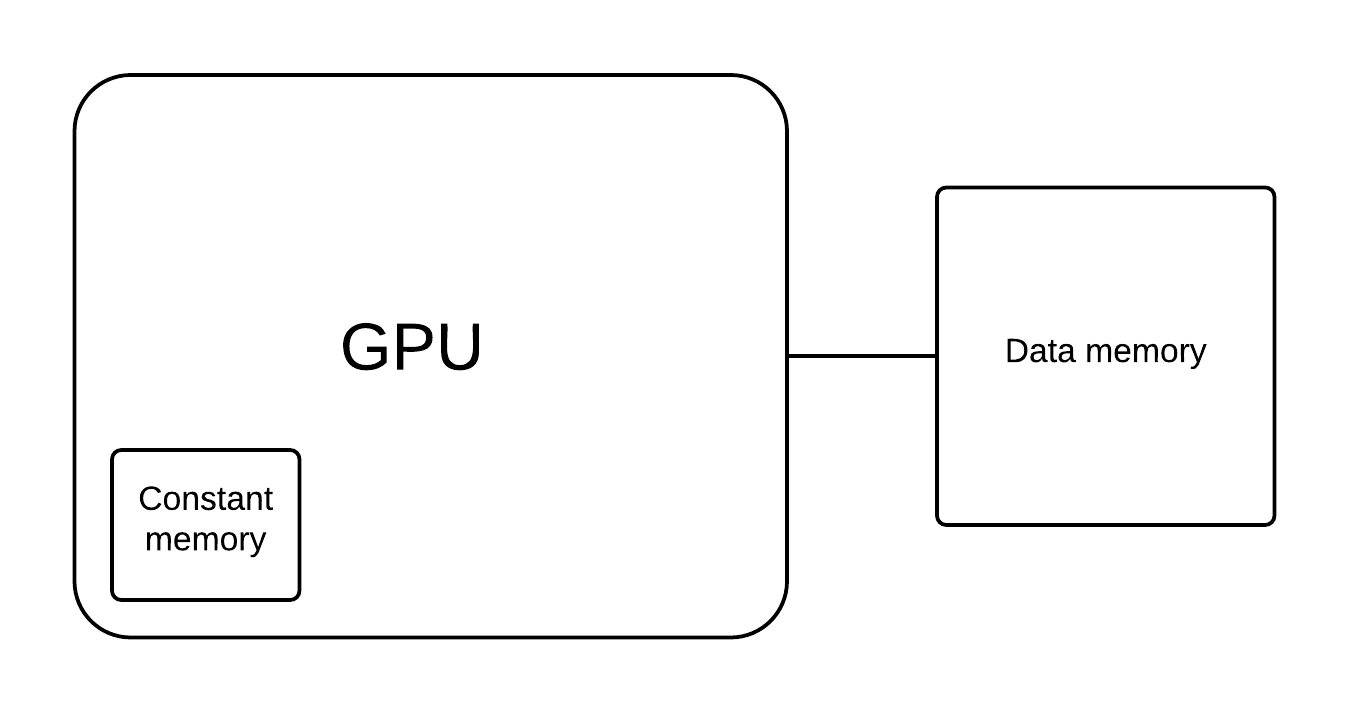
\includegraphics[width=\textwidth]{system_overview/diagrams/memory_overview.png}
	\caption{Overview of GPU memory architecture.}
	\label{fig:memory_overview}
\end{figure}

The Demolicious system contains two memories (Figure \ref{fig:memory_overview}), which the programmer can use.
The data memory is large, but has relatively high latency and low throughput.
Constant memory is small, but very fast.
It will typically be used for kernel parameters,
which will allow kernels to be re-used with varying output.
